%!TEX root = ../main.tex
%%%%%%%%%%%%%%%%%%%%%%%%%%%%%%%%%%
% Links:
%
% Difficulty: Companies: 
%%%%%%%%%%%%%%%%%%%%%%%%%%%%%%%%%%


%\begin{figure} \centering 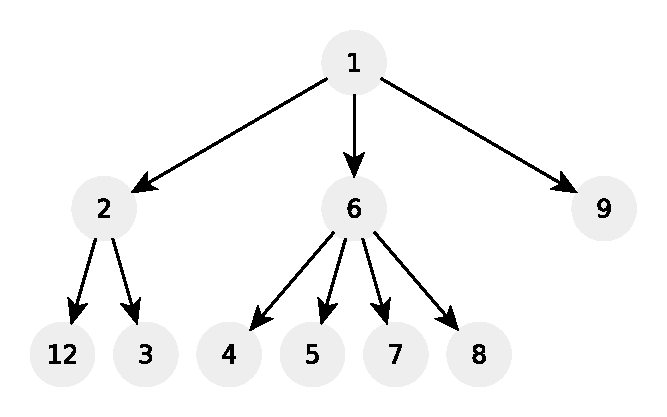
\includegraphics[width=\textwidth]{sources/nqueens/images/example1}
%   \caption[Sample short cpation]{Sample Caption}. \label{fig:nqueens:example1} \end{figure}

\chapter{N-Queens}
\label{ch:nqueens}
\section*{Introduction}
In this chapter we are going to discuss a problem that is more known because of one of its
specialization, namely the eight queen puzzle where you are challenged with the problem of placing
eight chess queens on an $8 \times 8$ chessboard so that no two queens threaten each other requiring,
therefore that no two queens share the same row, column or diagonal.

The n-queens is a classical and old problem which is used as an example of a simple but definitely 
non-trivial problem for various programming techniques such as constraint programming, 
logic programming , recursion and even genetic algorithms.
In the context of a programming interview, you should aim for precision and for outlining the solution strategy
clearly while solving it. The interview is very likely expecting you to be comfortable with the problem already, and possibly with the solution
but he want to see how well you can explain and materialize into code all the steps that are in between a purely brute-force and a more sophisticated solution.



\section{Problem statement}
\begin{exercise}
\label{example:nqueens:exercice1}

	%example1
	\begin{example}
		\label{example:nqueens:example1}
		\hfill \}
		
	\end{example}

	%example2
	\begin{example}
		\label{example:nqueens:example2}
		\hfill \
		
	\end{example}

	\begin{example}
		\hfill \
	
	\label{ex:nqueens:example3}
	\end{example}

	\begin{example}
		\hfill \

	\label{ex:nqueens:example4}	
	\end{example}
\end{exercise}

\section{Clarification Questions}

\begin{QandA}
	\item 
	\begin{answered}
		\textit{}
	\end{answered}
	
\end{QandA}

\section{Discussion}
\label{nqueens:sec:discussion}


\subsection{Brute-force}
\label{nqueens:sec:bruteforce}

\begin{minipage}{\linewidth}
	\lstinputlisting[language=c++, caption={Sample Caption},label=list:nqueens]{sources/nqueens/nqueens_solution1.cpp}
\end{minipage}

